

%Dati il layout di una metropolitana e la tabella orario dei treni che si vogliono far circolare. Viene definito il modello delle missioni dei singoli treni. Il modello delle missioni unito al modello dello stato della linea formano il modello di scheduling del sistema. 
%Il risultato dell'analisi del model chec ker 

In questo paragrafo viene descritto l'approccio utilizzato per verificare e correggere la presenza di deadlock in una metropolitana.

Il nostro approccio si basa sull'utilizzo iterativo di un model checker per verificare la presenza di deadlock di una metropolitana.

\begin{figure}[htp]
	\begin{centering}	
	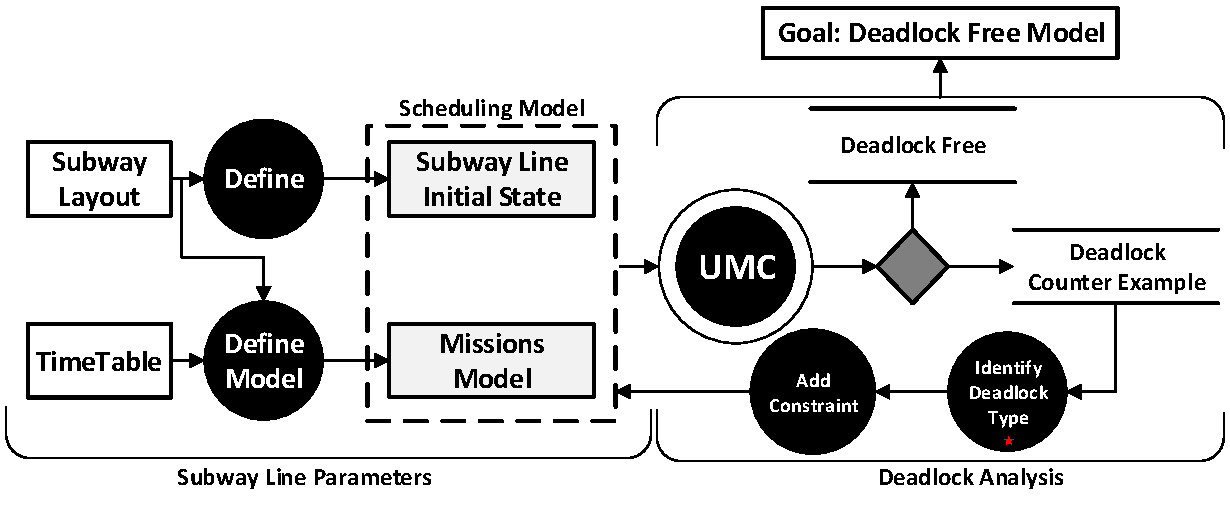
\includegraphics[width=0.45\textwidth, clip]{img/processo}
	\caption{Overview of the approach}
	\label{fig:process}
	\end{centering}
\end{figure}

Nella figura~\ref{fig:process} viene descritto graficamente l'approccio usato.

%%Nella prima fase, che chiamiamo SLP, vengo preparati i dati per effettuare l'analisi di deadlock della linea.
I dati di partenza sono  il layout della metropolitana e la tabella orario dei treni che si vogliono far circolare. Questi dati sono usati per definire
i modelli delle missioni dei singoli treni. 

Il layout della metropolitana viene usato anche per definire lo stato iniziale della linea. Cosi è possibile bloccare alcuni tratti di metropolitana perchè impegnate ad esempio da lavori di manutenzione.

I modelli di missione e lo stato iniziale della metropolitana costituiscono il modello di scheduling della metropolitana.


Il modello di scheduling viene analizzato tramite il model checker UMC[inserire riferimento]


Se risultato del modelchecker è controesempio di deadlock. Si identificano i pattern di deadlock e si inserisco delle nuove regole nelle aree scritiche identificate. 
Altrimenti il modelchecker verificherà la non presenza di casi di deadlock e quindi potremo affermare che il modello è libero di deadlock.
